% !TeX root = ../main.tex
% Add the above to each chapter to make compiling the PDF easier in some editors.

\chapter{Fake News Detection Models}\label{chapter:fnd_models}
The automated detection of fake news on social media comes with its characteristic challenges. First, the fact
that fake news are constructed to misguide its consumers makes them hard to distinguish by only using news content. Second, when we include social context into the model, the large-scale and noisy nature of social context data represents another issue~\parencite{HierarchicalPropagationNetworksForFND_Shu}. Moreover, from a broader perspective, fake news should be detected before it becomes widespread so that the amount of users affected can be minimized.\\
In this chapter, we examine how these challenges effect the model and dataset's design. We initially take a look at news content models in section~\ref{sec:newsContentModels}. In first section, we lay out the definitions for the materials used. After we give a detailed analysis of the dataset, we talk about the tokenizer and model itself, discuss its performance on the dataset. In section~\ref{sec:socialContextModels} we investigate social context based and hybrid models. Similar to the first section, we give definitons for the used material, then talk about the dataset and model. In this section, we also examine issues such as early fake news detection and model aging.\\

\section{News Content Models}
\label{sec:newsContentModels}
The majority of approaches for FND models utilizes news content. Models that base their predictions only on news content focus on the patterns in the text, especially words or word groups that appear frequently in other instances of the same class. As discussed in Section~\ref{sec:fakeNewsDetection}, there exist a variety of approaches available for news content models, however, due to unavailable or outdated datasets, we were unable to work with most news content models.

\subsection{Notation and Definitions}
\label{subsec:newsContentModels_Definitions}
Here we introduce the notation utilized in this section. Note that these notations will appear in its context, which will provide concrete examples for each symbol defined in Table~\ref{tab:newsContentModels_Notation}.\\
\begin{table}
    \begin{tabular}{cp{0.8\textwidth}}
        $x^{raw} \in X^{raw}$ & A news article.                                              \\
        $y^{raw} \in Y^{raw}$ & A label of news article.                                     \\
        $T$                   & Tokenizer function                                           \\
        $\psi$                & Label mapping function                                       \\
        $x^{tok} \in X^{tok}$ & Tokenized news article                                       \\
        $y \in Y$             & Vectorized class value.                                      \\
        $|x^{tok}|$           & The number of tokens in $x^{tok}$.                           \\
        $y^*$                 & Prediction of model.                                         \\
        $x \in X$             & Numeric vector of $x^{tok}$                                  \\
        $|x|$                 & The length of input vector                                   \\
        $l$                   & Index of a layer                                             \\
        $l_{embedding}$       & Embedding layer                                              \\
        $a_{i}^{(l)}$         & The value of unit $i$ in layer $l$                           \\
        $w_{ij}^{(l)}$        & Weight between units $i$ in layer $l$ and $j$ in layer $l+1$ \\
        $\sigma$              & Activation function                                          \\
    \end{tabular}
    \caption[Notation]{Notation used in this section.}
    \label{tab:newsContentModels_Notation}
\end{table}
Using this notation we now define some relevant concepts. First, we talk about terms and definitions for \emph{tokenization}, illustrate the mathematical insight in the tokenization process. First, to build upon a concrete foundation, let us consider a news article $x^{raw}$ fed to the tokenizer.
\begin{definition}[\emph{Tokenizer}]
    A tokenizer $T:X^{raw} \mapsto X^{tok}$ is a function that maps raw textual data to smaller units called tokens.
\end{definition}
A token can be a word, character or a subword. Therefore, we define three types of tokenization techniques:
\begin{itemize}
    \item \emph{Word tokenization} splits the given text into individual words based on a delimeter such as whitespace, commma, etc. This approach creates a vocabulary from the inputs it was trained on. All words do not appear in the vocabulary are replaced with unknown token ([UNK]), and this concept is called being \emph{Out Of Vocabulary}(OOV). Depending on the task, the size of the vocabulary can grow quite large. The solution for exploding vocabulary sizes was introduced in subword tokenization. The commonly used examples for word tokenizers are Word2Vec~\parencite{Word2Vec_Mikolov} and GloVe~\parencite{GloVe_Pennington}.
    \item \emph{Character tokenization} splits the text into single characters. Since the size of available characters is limited and known, the OOV problem is solved by encoding the unknown word by means of its characters. Although looks like a good solution, the length of tokens can be massive for long texts.
    \item \emph{Subword tokenization} splits the given text into subwords, also called \emph{n-gram characters}. For instance, comparative words like harder is segmented into hard-er, or superlative words like hardest is segmented into hard-est. The most common method for subword tokenization is \emph{Byte Pair Encoding} (BPE). BPE was introduced by~\cite{ANewAlgorithmForDataCompression_Gage} but adapted to word segmentation by~\cite{NeuralMachineTranslationOfRareWords_Sennrich}. BPE iteratively merges the most frequently appearing character or character sequences. This approach allows for an efficient space usage thus smaller vocabularies~\parencite{NeuralMachineTranslationOfRareWords_Sennrich}.
\end{itemize}
We say that an input is \emph{tokenized} after it is fed to the tokenizer. A tokenized news article $x^{tok}$ is a vector of tokens in which the order of the words and characters in $x^{raw} \in X^{raw}$ are kept. Furthermore, to get a fixed length output, we pad the tokenized sequence $x^{tok}$ with padding tokens ([PAD]) where the news article is not long enough. In case it is longer than the fixed length, then it is truncated. In case the sequence is padded, some tokenizer implementations in Huggingface use masks to mask out the pads so that they are not included in the computation. These are called masked transformers~\parencite{Transformers_Wolf}. In fact, our classifier has the same behavior which can be observed in~\ref{fig:InputPreProcessPipeline}.
\begin{center}
    $T(x^{raw}) = x^{tok} = [x_1^{tok}, \dots, x_n^{tok}]$, where $n = |x^{tok}|$.
\end{center}
Furthermore, we denote the space of raw label $Y^{raw} = \{"fake", "real"\}$, with
$y^{raw} \in Y^{raw}$. We use a label mapping function $\psi: Y^{raw} \mapsto Y$ that maps raw labels to classes, where $Y \in \mathbb{R}^2$ with,
\begin{center}
    \[\psi(y^{raw}) = y =
        \begin{cases}
            0, & y^{raw} = "fake" \\
            1, & y^{raw} = "real"
        \end{cases}
    \]
\end{center}
In order to feed the input to the model, we need numeric data which can be obtained by numerous techniques. One widely used approach is BoW representation which produces features based on the number of occurrences of a word or token. An alternative BoW representation uses the presence/absence of word instead of frequencies. A more sophisticated approach is \emph{Word2Vec}, which encodes words into numeric values by learning word associations. From the perspective of representation of a word, \emph{Word2Vec} can capture different degrees of similarity between words which allows for preservation of semantic and syntactic relationships~\parencite{Word2Vec_Mikolov}. It is clear that the transformation of words into numeric vectors is a very crucial stage for FND since we need to maintain as much contextual information as possible. Yet, the SOTA is an even more sophisticated approach called \emph{Transformer} which is utilized by many language models such as BERT. We will discuss Transformer architecture in~\ref{subsec:newsContentModels_TransformerArch}. For ease of the notation, we refer to this stage as \emph{Embedding Layer} and denote it with $l_{embedding}$.\\
The input transformation pipeline is illustrated in~\ref{fig:InputPreProcessPipeline}.
\begin{figure}
    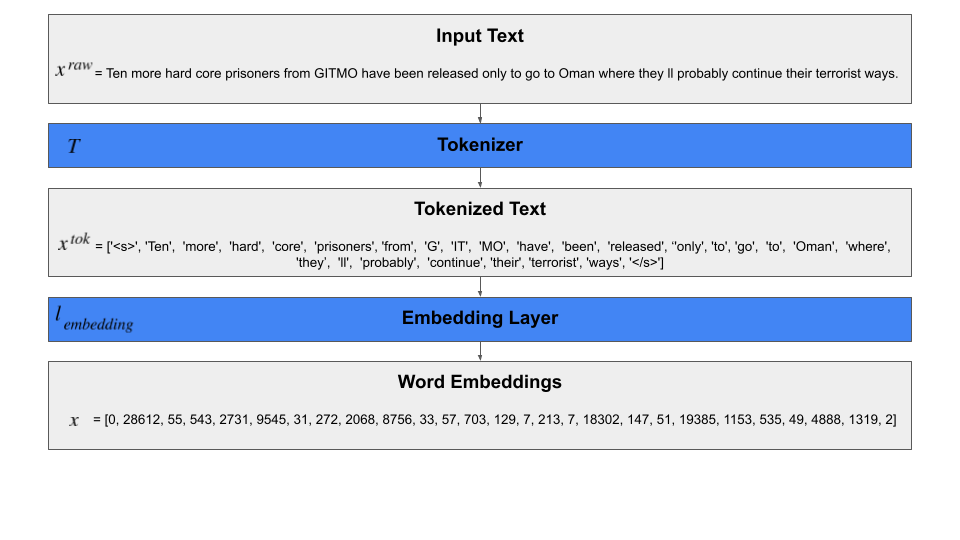
\includegraphics[scale=0.43]{InputPreProcessPipeline.png}
    \caption[The preprocessing pipeline for a textual input.]{The preprocessing pipeline for a textual input.}
    \label{fig:InputPreProcessPipeline}
\end{figure}
\begin{definition}[\emph{Classifier}]
    A classifier $f:X \mapsto Y$ is a function that outputs a predicted scores $f(x)_y$ for each class $y$ for a given input $x$.
\end{definition}
Our news content model is our classifier. It will predict whether a news piece is real or fake via assigning each label a probability.
\begin{definition}[\emph{Prediction}]
    A prediction $y^*$ is the maximum of predicted scores $f(x)_y$ of an FND classifier.
    \begin{center}
        $y^* = argmax_{y \in Y} f(x)_y$
    \end{center}
\end{definition}
We use a model that consists of several layers and a sophisticated architecture. Our model is able to work with big vocabularies and can classify news pieces based on various features.
\begin{definition}[\emph{Neural Network Classifier}]
    A neural network classifier is a \emph{classifier} $f$ that comprises of layers $l$ with $1 \leq l \leq L$, where $L$ denotes the number of layers. Each layer has a set of units $a_i^{(l)}$ with $i$ denoting the position of the unit in
    a layer $l$. We say that between two units $a_i^{(l)}$ belonging to layer $l$ and $a_j^{(l+1)}$ belonging to layer
    $l+1$ have a weight value $w_{ij}^{(l)}$ that connects them. Along with a non-linear activation function $\sigma$, we
    can define the value of the $j$-th unit $a_j^{(l+1)}$ in terms of weights and unit values from previous layer for an FCN, with $N$ is the number of units in layer $l$.
    \begin{center}
        $a_j^{(l+1)} = \sigma(\sum_{i=1}^{N} a_i^{(l)} w_{ij}^{(l)})$
    \end{center}
\end{definition}
Neural networks are very powerful models. They can train millions of parameters using matrix multiplications, gradient-based optimization methods and a fruitful set of other techniques, some of which will be discussed later.
\begin{figure}
    \centering
    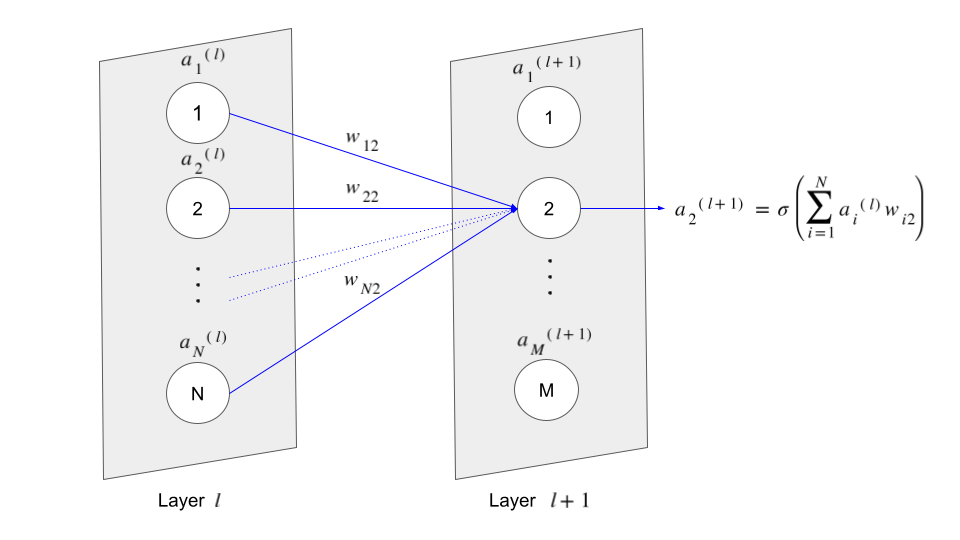
\includegraphics[scale=0.43]{NN_LayerRepresentation}
    \caption[Units and layers of an FCN]{Units and layers of an FCN. For brevity, arrows and weights are only drawn for $a_2^{(l+1)}$}
    \label{fig:NN_LayerRepresentation}
\end{figure}
Neural networks iteratively optimize the weights between layers such that the produced output is as close as to the
expected output. This is done so using optimization methods such as \emph{Gradient Descent} (GD)~\parencite{GD_Cauchy},
\emph{Stochastic Gradient Descent} (SGD)~\parencite{SGD_Robbins}, \emph{Adaptive Moment Estimation} (Adam)~\parencite{Adam_Kingma} to minimize the loss function. While there exist many optimization methods available for neural networks, we do not examine any of them.\\
For classification problems, we adopt a layer called \emph{Softmax}~\parencite{Softmax_Bridle} outputs the predicted scores $f(x)_y$ for each class $y$ by normalizing outputs $Z_y(x)$ from the previous layer.\\
\begin{center}
    $f(x)_y = \dfrac{exp(Z_y(x))}{\sum_{\hat{y} \in Y} exp(Z_{\hat{y}(x)})}$
\end{center}
The FCNs are the simplest architectures for neural networks. In an FCN, all units are connected which means there is a weight between each unit in layer $l$ and $l+1$. While very simple to construct, usage of these architectures when modeling sequences is not preferred due to the number of trained parameters such as weights and biases. Instead, when modeling sequences like sentences and documents, a common approach is RNNs which allow previous outputs to be used while having hidden states. However, RNNs are not powerful enough to represent long-term dependencies~\parencite{LearningLongTermDependenciesHard_Bengio} and suffer from vanishing/exploding gradients~\parencite{OnTheDifficultyOfTrainingRNNs_Pascanu}. Utilizing RNNs, an idea was proposed in which these shortcomings were addressed. Called \emph{Long Short-Term Memory} (LSTM)~\parencite{LSTM_Hochreiter}, the idea is to keep a cell state which is updated with previous cell's state. This cell state is conveyed to the consequent cells to form a chain that represents the document. More precisely, each cell corresponds to a token whose information will be shared with consequent tokens by the propagation of previously mentioned cell states. This approach is indeed very useful for long documents since news articles tend to be long and their sentences contextually relevant. LSTM is usually used in different variations based on the same idea. For instance, a consequent study has extended LSTMs with \emph{peephole connections} in~\parencite{LSTMPeephole_Gers}. LSTMs have been proven to deliver a good performance in NLP tasks such as \emph{speech recognitions}~\parencite{AchievingHumanParityinConvSR_Wayne}. LSTMs perform well however due to long training times and large memory requirements during training, they are being replaced with attention-based models.\\
One last thing to discuss is how the models are trained in terms of supervision. \emph{Supervised} models are trained with label data. \emph{Unsupervised} models work with unlabeled data and aims to find patterns in the data. A different setting is \emph{semi-supervised} models. These models are often provided with small amounts of labeled data and large amounts of unlabeled data for training. There are two settings for semi-supervised learning. \emph{Transductive} learning aims to predict unlabeled data whereas \emph{inductive} learning samples unlabeled data from the same distribution to
infer~\parencite{LearningByTransduction_Gammerman}. Having introduced all necessary notation and definitions, in ~\ref{subsec:newsContentModels_TransformerArch}, we discuss the SOTA approach the Transformer models which are based on attention mechanism.

\subsection{Transformer Architecture}
\label{subsec:newsContentModels_TransformerArch}
Transductive learning has been successfully utilized along with encoder-decoder structure in many language
tasks~\parencite{S2SLearningWithNNs_Sutskever, LearningPhraseRepresentations_Cho, AttentionIsAllYouNeed_Vaswani}. Transduction is first proposed in~\cite{LearningByTransduction_Gammerman} to counteract with unlabeled data problem.
In contrast to supervised learning, transductive learning does not require all data to be labeled, instead it utilizes
the clustered behavior of data. Using the gaps between different clusters and a small set of labeled data, transductive learning assigns labels to unlabeled data. Accordingly, Transformer models are transductive models and use encoder-decoder structure to achieve that.\\
Encoder-decoder structure that takes into account the order of words was proposed in~\parencite{LearningPhraseRepresentations_Cho}. This encoder-decoder structure consists of one RNN as encoder and one RNN as decoder. The encoder maps an input sequence to fixed-length vector, and the decoder maps this fixed-length vector to a target sequence. Transformer architecture adopts a similar approach which employs feed-forward and Multi-Head Attention layers in both encoder and decoder which is illustrated in Fig.~\ref{fig:transformerArchitecture} with N=6 stacks of encoders and decoders.\\
In order to reduce sequential computation, CNNs have been adopted as building blocks that parallelly compute hidden representations for all input and output positions~\parencite{AttentionIsAllYouNeed_Vaswani}. Although aimed to reduce computation, the number of operations to convey information from one random input or output to another increases linealy in ByteNet~\parencite{ByteNet_Kalchbrenner} and logarithmically in ConvS2S~\parencite{ConvS2S_Gehring}. Contrary to CNNs, Transformers are able to fix the number of operations by averaging attention-weighed positions which decreases the effective resolution. However, this decrease in resolution is neutralized by the utilization of Multi-Head Attention~\parencite{AttentionIsAllYouNeed_Vaswani}.
\begin{figure}
    \centering
    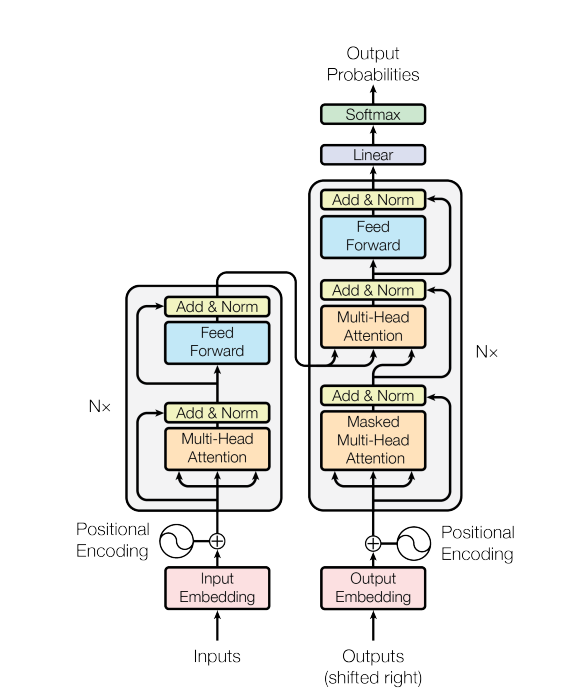
\includegraphics{TransformerArchitecture.png}
    \caption[The Transformer Model Architecture]{The Transformer Model Architecture (N=6). Figure obtained from~\parencite{AttentionIsAllYouNeed_Vaswani}}
    \label{fig:transformerArchitecture}
\end{figure}
Initially suggested in the decoder of the model proposed in~\parencite{NeuralMachineTranslationByJointlyLearning_Bahdanau}, an attention mechanism works similar to human attention; it learns to put more importance on some words that convey the relevant information about the sentence. It does so by means of a context vector that depends on a sequence of \emph{annotations}. An annotation $h_i$ for a word (or embedding) $x_i$ contains information about the complete input sentence but with a focus on the words that are closer to the word $x_i$. The context vector $c_i$ for word $x_i$ is obtained as a weighted sum of all these annotations $h_i$:
\begin{center}
    $c_i = \sum_{j=1}^{|x|} \alpha_{ij} h_j$.
\end{center}
The weight $\alpha_{ij}$ is obtained by applying softmax to associated energy $e_{ij}$ which is an output of the alignment model $a$. The alignment model $a$ is a feed forward neural network that jointly learns with the rest of the system. More precisely, we compute these values as follows:
\begin{center}
    $\alpha_{ij} = \dfrac{e_{ij}}{\sum_{k=1}^{|x|} exp(e_{ik})}$
\end{center}
where
\begin{center}
    $e_{ij} = a(s_{i-1}, h_j)$
\end{center}
with $s_i$ representing the current and $s_{i-1}$ the previous state of the
model~\parencite{NeuralMachineTranslationByJointlyLearning_Bahdanau}. This is called \emph{additive attention}.\\
For Transformer models, the authors define an attention function as \emph{mapping a query and a set of key-value pairs to an output, where the query, keys, values, and output are all vectors. The output is computed as a weighted sum of the values, where the weight assigned to each value is computed by a compability function of the query with the corresponding key.}~\parencite{AttentionIsAllYouNeed_Vaswani}. The Transformer model employs two different attention mechanisms, namely, \emph{Scaled Dot-Product Attention} and \emph{Multi-Head Attention}. Following~\parencite{AttentionIsAllYouNeed_Vaswani}, we denote that the input for the attention layers are matrices called queries $Q \in \mathbb{R}^{d_{model}xd_k}$, keys $K \in \mathbb{R}^{d_{model}xd_k}$, and values $V \in \mathbb{R}^{d_{model}xd_v}$, with $d_k$ as the number of keys or values and $d_{model}$ being the model dimension. Scaled Dot-Product Attention computes the dot product of all queries $q_i \in Q$ with all keys $K$ and scale the resulting wegihts with $\frac{1}{\sqrt{d_k}}$. After obtaining the softmax of the scaled weights, each weight is multiplied with the correspoding value to obtain attention values.
\begin{center}
    $Attention(Q, K, V) = softmax(\dfrac{QK^T}{\sqrt{d_k}})V$
\end{center}
The second attention mechanism, Multi-Head Attention, uses multiple attentions each of which uses a different learned linear projection of $Q$, $K$, $V$. Output of each of these attentions are then concatenated to obtain the final result. More precisely, it is computed as follows,
\begin{center}
    $MultiHead(Q, K, V) = Concat(head_1, head_2, \dots, head_h)W^{O}$
\end{center}
where each $head_i$ is calculated as,
\begin{center}
    $head_i = Attention(QW_i^Q, KW_i^K, VW_i^V)$
\end{center}
with projection for $Q$ as $W_i^Q \in \mathbb{R}^{d_{model}xd_k}$, $K$ as $W_i^K \in \mathbb{R}^{d_{model}xd_k}$, $Q$
as $W_i^V \in \mathbb{R}^{d_{model}xd_v}$, and lastly, $W^{O} \in \mathbb{R}^{hd_vxd_{model}}$~\parencite{AttentionIsAllYouNeed_Vaswani}.\\
We now discuss each part of the Transformer model briefly.\\
\begin{itemize}
    \item \emph{Encoder}: Consists of N=6 identical layers. Each of these layers have two sub-layers the first of which uses a Multi-Head Attention and layer normalization~\parencite{LayerNorm_Ba} along with a residual connection~\parencite{ResidualConnection_He} around. The second sub-layer consists of a feed-forward layer and layer normalization as well as a residual connection around the feed-forward layer~\parencite{AttentionIsAllYouNeed_Vaswani}
    \item \emph{Decoder}: Same as the encoder, this part is also composed of N=6 layers. Additional to the previously discussed two sub-layers in encoder, decoder adopts a third sub-layer which computes the attention values over the output of encoder. As it was done for encoder, decoder also utilizes layer normalization at the end of each sub-layer as well as the residual connection~\parencite{AttentionIsAllYouNeed_Vaswani}.
\end{itemize}
Each of the feed forward networks in the sub-layers are position-wise, meanining that they are applied to each position separately and identically. These feed-forward networks use different parameters for each layer. The embeddings are obtained through transductive learning. Lastly, the positional encodings for input embeddings are calculated using sine and cosine functions of different frequencies~\parencite{AttentionIsAllYouNeed_Vaswani}.\\
We have summarized the Transformers architecture in order to lay foundations for the model we use, DistilRoBERTa~\parencite{DistilBERT_Sanh, RoBERTa_Liu}. Next, we initially introduce details of BERT, then RoBERTa, and lastly DistilRoBERTa which is our news content model.

\subsection{Dataset }
\label{subsec:newsContentModels_Model}
We employ a fine-tuned version of case-sensitive Transformer model DistilRoBERTa\footnote{\url{https://huggingface.co/GonzaloA/distilroberta-base-finetuned-fakeNews}} for our task of FND with news content. DistilRoBERTa is a distilled version of \emph{A Robustly Optimized BERT Pretraining Approach} (RoBERTa)~\parencite{RoBERTa_Liu}. It uses the same distillation procedure adopted for  DistilBERT~\parencite{DistilBERT_Sanh} to \emph{Bidirectional Encoder Representations from Transformers} (BERT)~\parencite{BERT_Devlin}. This distillation procedure is referred to as \emph{Knowledge Distillation} and it compresses a model~\parencite{ModelCompression_Bucilua} - the teacher - by means of training a smaller model - the student - to reproduce the same behaviour~\parencite{DistillingTheKnowledge_Hinton}. In our case, the teacher is  RoBERTa and the student is DistilRoBERTa. First, in order to examine properties of RoBERTa, we discuss BERT in detail.\\
As the name suggests, the model architecture of BERT is a multi-layer bidirectional Transformer based on the Transformer model. BERT uses BookCorpus~\parencite{BookCorpus_Yukun} and English Wikipedia as training dataset, with two training objectives, \emph{Masked Language Modeling} (MLM) and \emph{Next Sentence Prediction} (NSP). MLM procedure applies the following for each sentence sampled from a document in the cumulative dataset.
\begin{itemize}
    \item Mask 15\% of the tokens.
    \item In 80\% of the cases, replace the masked tokens with [MASK].
    \item In 10\% of the cases, replace the masked tokens with a different random vocabulary token.
    \item In the remaining 10\% of the cases, the masked tokens are left unchanged.
\end{itemize}
NSP procedure is a binary classification loss that predicts whether two segments (sequences of tokens) are consecutive in
the original text. \emph{Positive} and \emph{negative} examples are sampled with equal probability in this process.
Positive examples are created with taking the consecutive sentences from the text corpus, whereas negative examples
are generated by pairing segments from different documents~\parencite{RoBERTa_Liu}.\\
RoBERTa is an optimized, longer pretrained with longer sequences version of a BERT implementation that uses only MLM
as training objective. Contrary to BERT, RoBERTa keeps a dynamic masking pattern that changes in training. It is
pretrained on reunion of five datasets (three more datasets than BERT) that size up to 160 gigabytes (GB): BookCorpus~\parencite{BookCorpus_Yukun},
English Wikipedia~\parencite{EnglishWikipedia_Wiki},
CC-News~\parencite{CCNews_Nagel}, OpenWebText~\parencite{OpenWebText_Radford},
Stories~\parencite{ASimpleMethodForCommonsenseReasoning_Trinh}.\\
RoBERTa tokenizes texts using BPE with a vocabulary size of 50,000 and maximum sequence length (maximum number of tokens) as 512. The beginning and end of each document (news article) is marked with <s> and </s> respectively. With MLM as training objective and Adam~\parencite*{Adam_Kingma} as the optimizer, the model reaches better results than BERT. Additionally, it should be noted that since these models are further trained for downstream tasks, thus we refer to training stage as pretraining to avoid any confusion. \\
DistilRoBERTa has the same general architecture as RoBERTa but the number of layers are reduced by a factor of two, the
\emph{token-type embeddings} and the pooler are removed. Then DistilRoBERTa is initialized with layers from the teacher.
The distillation is done with very large batches~\parencite{DistilBERT_Sanh}. Using RoBERTa as a teacher, the student DistilRoBERTa is pretrained on OpenWebTextCorpus~\parencite{OpenWebTextCorpus_Gokaslan} a reproduction of OpenWebText~\parencite{OpenWebText_Radford}.\\
Our fine-tuned DistilRoBERTa was trained on a dataset\footnote{\url{https://huggingface.co/datasets/GonzaloA/fake_news}} curated from different sources. Although there exist better datasets and news content models, we opted for this particular model for two reasons. First, most SOTA news content models do not provide their code and dataset to reproduce results. Second, since Transformers are SOTA and this particular trained model provides us with not only the dataset but also with the train/test/validation splits which allows us to analyze its explanation. Now, we analyze the dataset, convey the distribution of labels and discuss potential peculiarities. Then we talk about the performance of the model, and reason about it.\\
\textbf{Dataset.} The news content dataset comprises of 40587 samples whose distribution of labels and train/validation/test splits are provided in Fig~\ref{fig:DatasetDistributionByLabelAndSplit}. The proportion of fake news is 46\%, which is a fair distribution between real and fake news instances. The train/validation/test split is 60\%/20\%/20\% which is common practice.
\begin{figure}
    \centering
    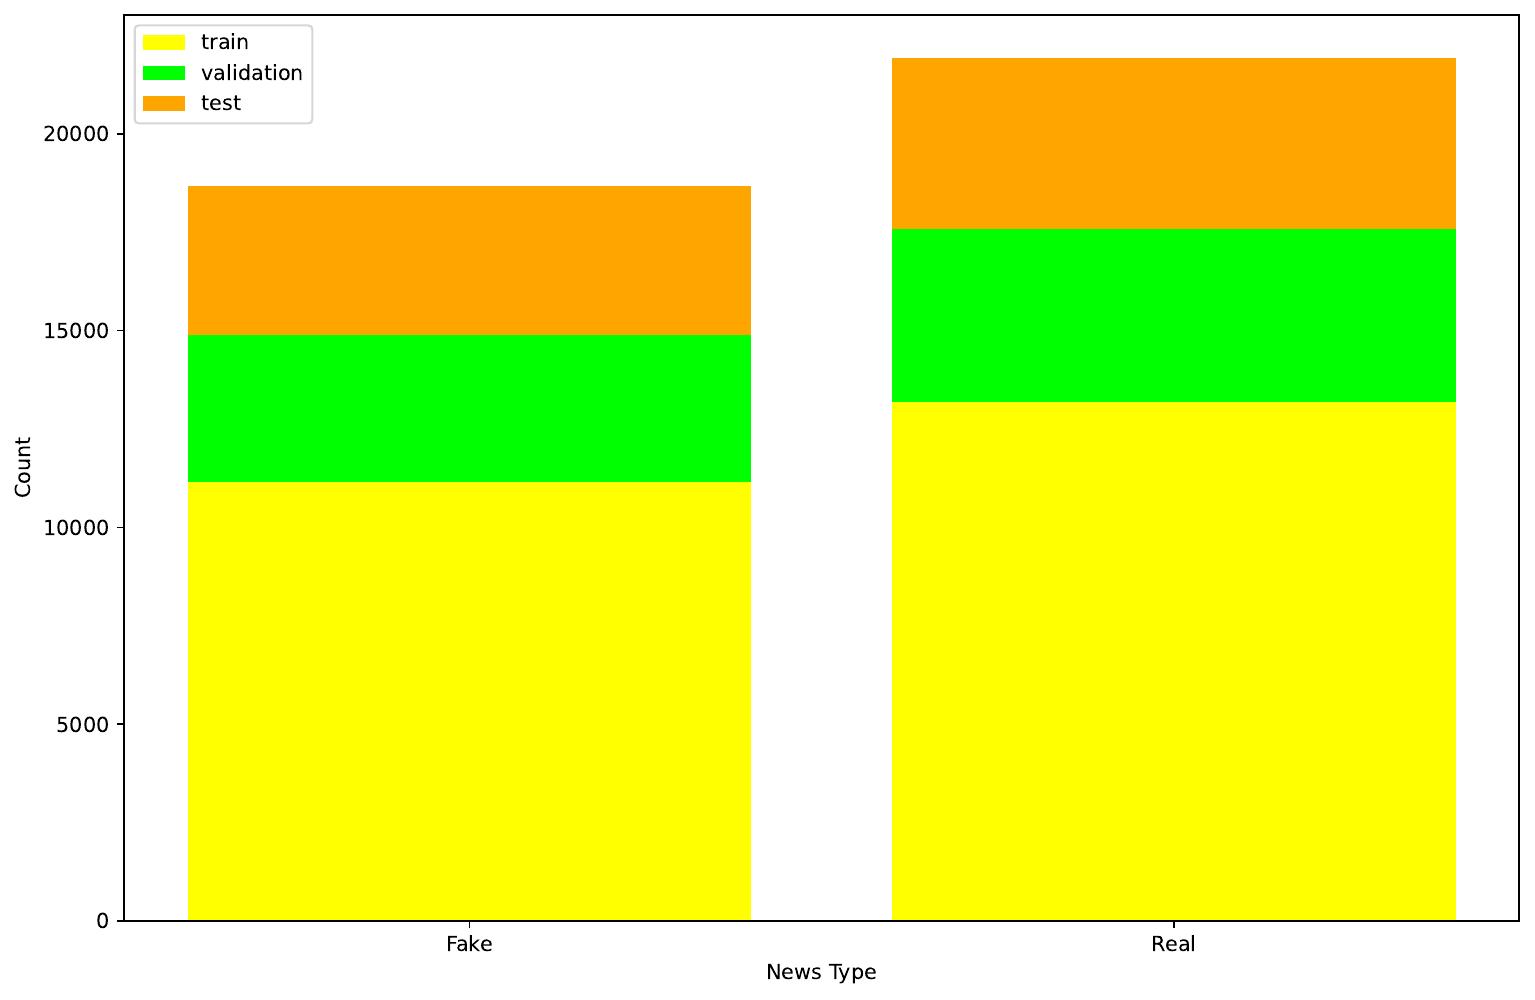
\includegraphics[scale=0.5]{DatasetDistributionByLabelAndSplit}
    \caption[News content dataset distribution by label and train/validation/test split]{News content dataset distribution by label and train/validation/test split}
    \label{fig:DatasetDistributionByLabelAndSplit}
\end{figure}
We analyze 500 most frequently occurring tokens in the dataset using a WordCloud~\parencite{WordCloud_Oesper} visualization for all samples of real and fake news separately in Fig~\ref{fig:WordCloudVisualizations}. From the visualization, we can observe that samples from both datasets contain the words \emph{new}, \emph{state}, \emph{President}, \emph{Republican}. In fact, 500 most frequent tokens from fake news samples and real news samples share 63\% of tokens. Furhtermore, we observe that one of the most frequent token is \emph{Reuters} in real news instances. In fact, 95.93\% of real news samples contain the keyword \emph{(Reuters)}. This might be give rise to a problem where the model learns the real news instances based on a couple tokens like \emph{(}, \emph{Reuters}, \emph{)}. This will be analyzed in detail in Section~\ref{sec:explainabilityOfNewsContentModels}.
\pagebreak
\begin{figure}
    \centering
    \subfloat[Fake news]{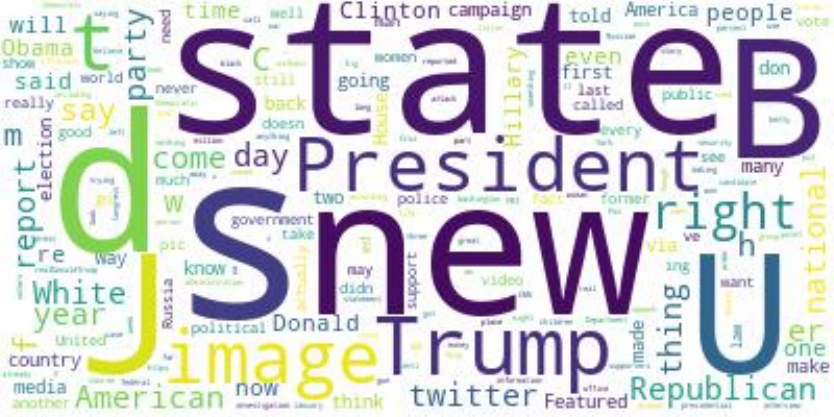
\includegraphics[width=0.45\textwidth]{DatasetFakeFrequentTokensWordCloud.png}\label{subfig:WordCloud_DatasetFakeFrequentTokensWordCloud}}
    \hfill
    \subfloat[Real news]{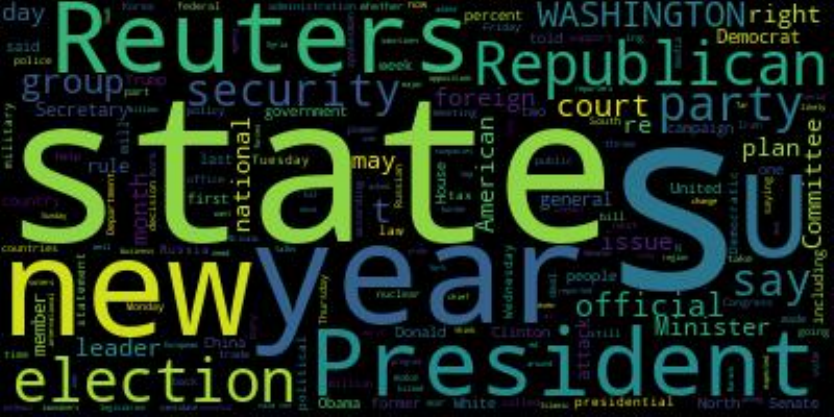
\includegraphics[width=0.45\textwidth]{DatasetRealFrequentTokensWordCloud.png}\label{subfig:WordCloud_DatasetRealFrequentTokensWordCloud}}
    \caption[WordCloud visualiations for most frequently occurring 500 tokens in both classes]{WordCloud visualiations for most frequently occurring 500 tokens in samples of both classes}
    \label{fig:WordCloudVisualizations}
\end{figure}\\
\textbf{Training.} Huggingface provides us with a \emph{TextClassificationPipeline} which allows to feed the dataset from Huggingface directly\parencite{Transformers_Wolf}. This pipeline includes the tokenization process and the embedding layer before feeding it to our classifier. Our classifier has 6 layers, 12 attention heads and  hidden size of 768 that totals up to 82M parameters (RoBERTa has 125M parameters). The vocabulary size is 50265 including special tokens. The model also uses a technique called \emph{dropout} which is a regularization technique that drops some connections between layers based on a probability value~\parencite{Dropout_Nitish}. All model parameters are defined in~\ref{tab:newsContentModelParameters}.\\
\begin{table}
    \centering
    \begin{tabular}{|l|l|}
        \hline
        Attention dropout probability           & 0.1                             \\
        \hline
        Classifier dropout                      & None                            \\
        \hline
        Hidden layer activation function        & GELU~\parencite{GELU_Hendrycks} \\
        \hline
        Hidden size                             & 768                             \\
        \hline
        Intermediate size                       & 3072                            \\
        \hline
        Layer normalization factor ($\epsilon$) & 1e-05                           \\
        \hline
        Maximum position embeddings             & 514                             \\
        \hline
        Number of attention heads               & 12                              \\
        \hline
        Number of layers                        & 6                               \\
        \hline
        Vocabulary size                         & 50265                           \\
        \hline
    \end{tabular}
    \caption[Parameters of news content model]{Parameters of news content model}
    \label{tab:newsContentModelParameters}
\end{table}
Note that maximum position embeddings parameter also considers document start and end tokens when reporting its length. When feeding tokens $x^{tok}$ to the model, the start (<s>) and end (</s>) tokens are added by the model pipeline, so this leaves us with maximum sequence length of 512, i.e., $|x|=512$. Note that in Figure~\ref{fig:InputPreProcessPipeline} the length of $x$ is not 512 since the paddings are masked out before feeding the input $x$ to the model.   Model is trained for 3 epochs with a batch size of 16, Adam ($\beta_1=0.9$, $\beta_2=0.999$, $\epsilon=1e-08$) as the optimizer and a linear learning rate scheduler. The performance metrics for the model is provided in Table~\ref{tab:newsContentModelPerformanceMetrics}.\\
\begin{table}
    \centering
    \begin{tabular}{c | c | c | c}
        Accuracy & Precision & Recall  & F1 score \\
        98.85\%  & 98.82\%   & 99.03\% & 98.92\%  \\
    \end{tabular}
    \caption[The performance metrics for news content model.]{The performance metrics for news content model.}
    \label{tab:newsContentModelPerformanceMetrics}
\end{table}
The model performs very well on the dataset. Only 4 samples out of 8117 are classified incorrectly in the test split of the dataset. We will closely work with those 4 samples when explaining our model and inspect the reasons behind this performance in Section~\ref{sec:explainabilityOfNewsContentModels}.\\
We have laid out the foundations for the model we used, reported the characterstics, training details, and performance of the news content model in this section. Although seems powerful in this case, usually news content models are easily outdated as the structure of news changes rapidly and fake news fabricators can replicate the properties that can be seen in real news content~\parencite{HierarchicalPropagationNetworksForFND_Shu}. Thus, we consider a different approach which primarily considers social context features for FND.\\

\section{Social Context Models}
\label{sec:socialContextModels}
As discussed in Section~\ref{sec:fakeNewsDetection}, social media's interconnected nature leads to fast dissemination of
fake news. When a news piece is shared, it cascades through social media by means of friendship networks. These networks
can be exploited to gather information about how fake news spread. Moreover, a user's historical information can prove effective when trying to analyze whether a news piece is real or not. This assumption stems from the psychological facts we discussed in Section~\ref{sec:fakeNewsDetection}. To recap, if a user is sharing fake news most of the time, i.e., the user's tweets are marked as fake, then it is likely that the next news piece they share would be fake as well. Usually, fake news are shared most within echo chambers, which gives rise to quick spread of fake news.\\
There exist many different approaches for social context models, however, it is a long and challenging task to create a dataset for social context models as the amount of data to be collected can grow dramatically. Thus, we selected a dataset that provides us with the social context information as well as the news content. Being a graph dataset, \emph{User Preference-aware Fake Detection} (UPFD)~\parencite{UPFD_Dataset_Shu} builds a propagation tree for the news. But in order to build a model that takes graphs as input we can no longer rely on standard deep learning approaches as the graph data has a different structure than news content data. It holds node information as well as edge information between nodes, allowing to store rich relational data~\parencite{UPFD_Dataset_Shu}.\\
In this section, we lay out foundations for the dataset and GNNs we used. Then we talk about the social context models along with their dataset UPFD that we used in this thesis. We also give some insights from~\parencite{HierarchicalPropagationNetworksForFND_Shu} in which the authors of UPFD dataset analyze the data they later utilized to create the graph dataset UPFD.\\

\subsection{Overview of Graphs}
In this section, we introduce definitions to cover graphs and different types of GNNs. But we do not discuss each model type in detail due to GNNs' extensive background. Thus, we do not provide a notation for this section but we give mathematical definitions when required.\\
Graphs are an example of \emph{non-euclidean} data, meaning that in contrast to \emph{euclidean} data, they can represent complex relations and entities more accurate than one or two dimensional representations. Non-euclidean data used in GDL can be grouped into grids, graphs, groups, geosedics, and gauges, which are also called the 5G's of \emph{Geometric Deep Learning} (GDL)~\parencite{GeometricDeepLearning_Bronstein}. We are interested in one G only, graphs.
\begin{definition}[\emph{Geometric Deep Learning (GDL)}]
    A class of deep learning that aims to build models that can learn to predict on the non-euclidean domain.
\end{definition}
GDL is an extensive field covering various techniques that can be appied to non-euclidean domain. Due to its complex nature, we do not provide a rigorous background on GDL. For a detailed background on GDL, we refer the reader to an extensive study on GDL~\parencite{GeometricDeepLearning_Bronstein}. We only discuss parts related to GNNs that we utilized. First we define a graph.
\begin{definition}[\emph{Graph}]
    A graph is a non-euclidean type of data that represents the relations between entities.
\end{definition}
From the perspective of individual node connections, graphs can be categorized into two classes, \emph{directed} and \emph{undirected} graphs. Directed graphs have direction information in their edges, i.e., the information flows strictly from one node to another. On the other hand, undirected graphs do not have this limitation, the information flow is bidirectional. Since we are only interested in undirected graphs like our dataset, we give preliminaries for an undirected graph.\\
Following common notation on graphs, we define an undirected graph as $\mathcal{G} = (\mathcal{V}, \mathcal{E})$ with $\mathcal{V}$ as the set of nodes and $\mathcal{E}$ as the set of edges in a graph $\mathcal{G}$. We say that an edge $(v_i, v_j)$ exists between two nodes $v_i$ and $v_j$. Moreover, from the perspective of a graph's connectedness, there exist two types of graphs, \emph{cyclic} or \emph{acycylic}. Simply put, cyclic graphs have cycles in them, i.e., the graphs allows for at least one node $v_i$ to have a series of different edges that creates a cycle back to the node $v_i$. In contrast, acyclic graphs do not contain cycles. A concrete example for undirected acyclic graphs are trees. Also the structure of our dataset, trees have strictly one edge between two nodes.\\
When we look at graphs from node and edge type, we classify graphs as \emph{homogeneous} and \emph{heterogeneous} graphs. Homogeneous graphs have nodes and edges of the same type, whereas heterogeneous graphs have different types of nodes and edges. One example for homogeneous graphs are social networks in which the nodes are users and the edges represent the friendship between two users. If we modify this social network into a more detailed version in which we choose to represent another relationship between users, such as colleagueship, then we would have a heterogeneous graph, because there would be two types of edges in the graph.\\
Finally, if we consider graphs from a temporal aspect, we observe two kinds of graphs, \emph{static} and \emph{dynamic}. Static graphs stay the same over time, their topology or features do not change. In contrast, dynamic graphs' features and topology vary  over time, thus making time an important factor when working with dynamic graphs.

\subsection{Graph Neural Networks}
GNNs are neural networks that can take graphs as an input and produce predictions at three different levels:
\emph{node-level}, \emph{edge-level}, and \emph{graph-level}. Node-level tasks include node classification, node
regression, node clustering. Node classification aims to categorize nodes into classes. Node regression deals with
predicting continuous value for each node. Lastly, node clustering aims to group nodes into several clusters. Edge-level tasks consist of edge classification and link prediction. Edge classification tries to categorize an edge. Link prediction aims to find whether there is an edge between two nodes. Graph-level predictions are graph classification, graph regression, and graph matching. In all these settings, the model needs to learn representations of graph~\parencite{GNNsAReview_Zhou}.\\
In our experiments, we used two different models one of which uses a convolutional layer called GraphSAGE~\parencite{GraphSAGE_Hamilton} and the other uses a convolutional attention layer called \emph{Graph Attention} (GAT)~\parencite{GraphAttentionNetworks_Velickovic}. Here we give background for both but we do not dive into details. We first give information about general framework.\\
\cite{GNNsAReview_Zhou} defines three modules that are involved in a generic GNN model: \emph{propagation module}, \emph{sampling module}, \emph{pooling module}. Propagation module deals with information propagation between nodes so that the aggregated information can represent features and topology of the graph. Propagation modules usually employ a \emph{convolution operator} or \emph{recurrent operator} to aggregate information from neighbors of nodes separately. These aggregated values are then used to update the representation of the nodes, edges, and graph. Additionally these modules employ a skip connection that helps collect previous representations of nodes to alleviate the over-smoothing problem. Sampling module is used when the input graph is large to handle propagation. It is used before propagation module. Lastly, pooling modules are employed when we need to extract information to represent high-level graphs.\\
We will mostly deal with propagation module and the operations within. We do not dive into mathematical background of convolutions in detail but we introduce mathematical formulations in order to illustrate the operations our models are using. Also, we do not discuss recurrent operations on graphs as their background is extensive and out of scope of this thesis. We refer the reader to~\cite{GNNsAReview_Zhou} for an extensive mathematical baackground on convolutions and other operations on spectral domain. However, we will summarize the behavior of convolutions on graphs in order to give the sufficient knwoledge for the models we used.\\
\textbf{Convolutions on graphs.} The idea of convolution operators is to generalize convolutions from another domain to spectral domain. In general there are two types of convolutional operations.\\
The first, \emph{spectral approaches}, are based on graph signal processing and defines its convolutional operators in the spectral domain~\parencite{TheEmergingFieldOfSignalProcessingOnGraphs_Shuman}. Spectral methods initially transform a graph signal $x$ to the spectral domain by the graph Fourier transform $\mathcal{F}$, then the convolution operation is applied. The output from convolution is transformed back with the inverse Fourier transform $\mathcal{F}^{-1}$. Now we summarize the mathematics behind this approach in order to convey our models' characteristics. Graph Fourier and inverse graph Fourier transform are defined as,
\begin{center}
    $\mathcal{F}(x) = U^T x$
\end{center}
\begin{center}
    $\mathcal{F}^{-1}(x) = Ux$
\end{center}
where $U$ is the eigenvalue matrix of normalized graph Laplacian $L = I_N - D^{\frac{-1}{2}} A D^{\frac{-1}{2}}$ with $I_N$ the identity matrix of dimension $N$, $D$ as the degree matrix and $A$ as the adjacency matrix of the graph. $L$ is a real symmetric positive semi-definite matrix which helps us with factorization $L = U \Lambda U^T$ where $\Lambda$ denotes the diagonal eigenvalue matrix~\parencite{GNNsAReview_Zhou}. Now that we can convert our graph signal $x$ to spectral domain and back, following~\cite{AWaveletTourOfSignalProcessing_Mallat} and~\cite{GNNsAReview_Zhou}, we can define the convolution operation on $x$.
\begin{center}
    $g \star x = \mathcal{F}^{-1}(\mathcal{F}(g) \bigodot \mathcal{F}(x))$ \\ $= U(U^T g \bigodot U^T x)$
\end{center}
where $\bigodot$ stands for element-wise multiplication and $U^Tg$ is the convolution filter in the spectral domain. This can be further simplified into the basis function of spectral methods:
\begin{center}
    $g_w \star x = U g_w U^T x$
\end{center}
where $g_w$ is a diagonal learnable matrix. Essentially, all spectral methods use a convolutional filter $g_w$ but their choice of design creates a variety of approaches that are built upon each other. We only discuss the ones necessary for our models. The main idea of modern convolutional operators come from approximating $g_w$ with $k$-th order Chebsyshev polynomials. GCN adopts $k=1$ to avoid overfitting. Moreover, it introduces a renormalization trick to solve the exploding/vanishing gradient problem~\parencite{GCN_Kipf}. Further works like AGCN~\parencite{AGCN_Li} have employed a similar approach. Additionally, GCN is employed to an extent in spatial approaches.\\
The second, \emph{spatial approaches} focus on the graph structure. They define convolutions directly on graph topology. Spatial approaches can be grouped into \emph{basic}, \emph{attention-based}, and \emph{framework}. Basic spatial approaches define convolution operations on the neighborhoods of different sizes. Neighborhoods are defined based on nodes as follows $\mathcal{N}_v$ for a node $v$. There exist several basic spatial approaches such as the diffusion CNN (DCNN)~\parencite{DCNN_Atwood} which describes the neighborhhood for nodes using transition matrices, the learnable GCN (LGCN)~\parencite{LGCN_Gao} which utilizes CNNs as aggregators by applying max pooling on neighborhhood matrices.\\
Another example, GraphSAGE uses an inductive learning approach to sample then aggregate features from a node's local neighborhhood. GraphSAGE uniformly samples a fixed-size collection of neighbors then aggregates this collection to produce embeddings for the graph~\parencite{GraphSAGE_Hamilton}. More precisely, let us assume that we have learned the parameters of $K$ aggregator functions denoted as $\textsc{AGG}_k$, and a set of weight matrices $W^k$ where $\forall k \in \{1, \dots K\}$. $k$ can be referred to as layer or search depth. Then for each $k$ we go through all nodes $v \in \mathcal{V}$ and apply an aggregation then an update. Concretely, at each $k$ and at each $v$, let $h_v^{k-1}$ denote the hidden state of a node $v$ at layer $k-1$. Following the same notation, we refer to the hidden state of a node's neighborhood $\mathcal{N}_v$ at layer $k$ as $h_{\mathcal{N}_v}^k$. GraphSAGE formalizes its aggregation and update operation at layer $k$ as:
\begin{center}
    $h_{\mathcal{N}_v}^{k} = \textsc{AGG}_{k}(\{h_u^{k-1}, \forall u \in \mathcal{N}_v\})$
\end{center}
\begin{center}
    $h_v^k = \sigma(W^k [h_v^{k-1} || h_{\mathcal{N}_v}^k])$
\end{center}
where $||$ denotes concatenation of two vectors, $[h_v^{k-1} || h_{\mathcal{N}_v}^k]$ concatenated vector and $\sigma$
a non-linear activation function. GraphSAGE employs three different aggregators: \emph{mean aggregator}, \emph{LSTM aggregator}, and \emph{pooling aggregator}. Mean aggregator collects sampled neighborhood information and takes the element-wise mean of the vector set $\{h_u^{k-1}, \forall u \in \mathcal{N}_v\}$. The inductive version also includes previous layer representation of node $v$, $h_v^{k-1}$. LSTM aggregator uses an LSTM to collect neighborhood information. LSTMs are more expressive than mean aggregators. However, since LSTMs are not permutation invariant, i.e., they process
their inputs sequentially, they need a modification to work with unordered sets. Finally, pooling aggregator first independently feeds each neighbor's vector to a FCN, then apply a pooling operation on the output.\\
The third, \emph{attention-based approaches}, utilizes the same attention logic introduced in~\ref{subsec:newsContentModels_TransformerArch} by following~\cite{NeuralMachineTranslationByJointlyLearning_Bahdanau}. A recent work Graph Attention Networks (GAT)~\parencite{GraphAttentionNetworks_Velickovic} proposes to integrate attention into the propagation step by computing the hidden state for node $v$ at layer $k$ as follows:
\begin{center}
    $h_v^{k} = \sigma(\sum_{u \in \mathcal{N}_v} a_{vu} W h_u^k)$ \\
\end{center}
\begin{center}
    $\alpha_{vu} = \dfrac{exp(LeakyReLU(a^T[Wh_v || Wh_u]))}{\sum_{k \in \mathcal{N}_v}exp(LeakyReLU(a^T[W h_v || W h_k]))}$
\end{center}
with $W$ as the weight matrix, $a$ as the weight vector of feed forward network and the non-linear activation function LeakyReLU is defined as:
\begin{center}
    \[LeakyReLU(\gamma, x) =
        \begin{cases}
            x,          & if x \geq 0 \\
            \gamma * x, & otherwise   \\
        \end{cases}
    \]
\end{center}
The authors in~\cite{GraphAttentionNetworks_Velickovic} also utilize Multi-Head Attention in order to stabilize the
learning process of attention(also called self-attention or intra-attention)~\parencite{AttentionIsAllYouNeed_Vaswani}. Concretely, same as GraphSAGE defined $K$ aggregators, GAT defines $T$ independent attention heads to compute hidden states and then features of these hidden states are either concatenated,
\begin{center}
    $h_v^k = ||_{t=1}^T \sigma(\sum \alpha_{vu}^t W_t h_u^k)$
\end{center}
or averaged,
\begin{center}
    $h_v^k = \sigma(\frac{1}{T} \sum_{t=1}^T \sum_{u \in \mathcal{N}_v} \alpha_{vu}^t W_t h_u^k)$
\end{center}
to obtain the output where $\alpha_{vu}^t$ represents the normalized attention values of the attention head $t$.\\
The last convolutional spatial approaches cover general frameworks that aims to integrate multiple different models into one framework. A mixture model MoNet was proposed by~\cite{GeometricDeepLearningOnGraphsAndManifolds_Monti} which is a spatial framework for unifying models such as GCN~\cite{GCN_Kipf}, ~\cite{GeodesicCNNsOnRiemannManifolds_Masci}, DCNN~\cite{DCNN_Atwood} and many more in non-euclidean domain.\\
One more thing we need to investigate is graph sampling in order to cover everything that was utilized in this thesis. GNN models suffer from an issue called \emph{neighbor explosion} which stems from having massive sizes of supporting neighbors from all previous layers as the number of layers increases~\cite{GNNsAReview_Zhou}. Likewise, as graph size increases, we will encounter the same problem. Sampling is used to solve this issue and it can be done on three levels: \emph{node sampling}, \emph{layer sampling}, and \emph{subgraph sampling}. Node sampling creates a subset using the neighborhood set $\mathcal{N}_v$ of the node's $v$. As discussed previously, GraphSAGE~\parencite{GraphSAGE_Hamilton} employs node sampling. Layer sampling takes a different approach and it selects a subset of nodes for aggregation. Lastly, subgraph sampling deals with the graph as a whole. One approach is to use clustering algorithms to obtain these subgraphs~\parencite{ClusterGCN_Chiang}. Another is to sample nodes and edges from graph to create a subgraph~\parencite{GraphSAINT_Zeng}.\\

\subsection{Dataset and Models}
FakeNewsNet, UPFD, explain the dataset, no of edges/nodes. Which models use this dataset,

\section{Early Fake News Detection and Model Aging}